\clearpage\begingroup\SourceLeaf{67c}\HistoricalHead{62}{L}{PHYSIK. NACHLASS.}
\begin{center}[5.]\end{center}
\noindent{\small [S. 187]}
\begin{center}\textbf{Ruhige Hinüberführung zu einem andern Gleichgewichtszustand.}\end{center}
\noindent\hspace*{\parindent}\begin{tabular}{@{}l@{}}
Zwei Zeitintervalle \(t,t'\)\\
Schwingungsdauer \(T\)\\
Logarithmisches Decrement \(\lambda\)[\textsuperscript{***})]\\
\(R\) Quadrant
\end{tabular}
\begingroup\renewcommand{\thefootnote}{}\footnotetext{[\textsuperscript{***}) In der Handschrift steht »Halbes logarithmisches Decrement«.]}\endgroup
\clearpage\SourceLeaf{68a}\HistoricalHead{63}{R}{BERECHNUNG MAGNETISCHER KRÄFTE.}
\indent Es sei
\[
P=\frac{2Rt}{T},\quad Q=\frac{2Rt'}{T}\text{[\textsuperscript{*})]},
\]
\begingroup\renewcommand{\thefootnote}{}\footnotetext{\(\Bigl[\)\textsuperscript{*}) In der Handschrift steht \(Q=\dfrac{2Rt}{T}.\Bigr]\)}\endgroup
\[
\log p=-\frac{\lambda}{[2R]}P,\quad\log q=+\frac{\lambda}{[2R]}Q,
\]
\noindent Gleichungen:
\[
\begin{aligned}
p\cos P+q\cos Q&=1,\\
p\sin P&=q\sin Q.
\end{aligned}
\]
\begin{center}
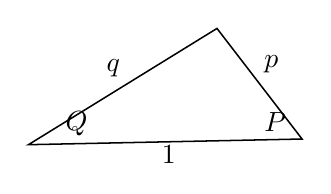
\begin{tikzpicture}[x=.018cm,y=.018cm,line width=.55pt]
\draw (0,0)--(133,82)--(193,4)--cycle;
\node[above left,inner sep=1pt] at (67,45) {$q$};
\node[above right,inner sep=1pt] at (164,48) {$p$};
\node[below,inner sep=1pt] at (99,2) {$1$};
\node at (34,15) {$Q$};\node at (174,16) {$P$};
\end{tikzpicture}
\end{center}
\noindent Daraus
\[
\frac{1+pp-qq}{2p}=\cos P,\quad
\frac{1+qq-pp}{2q}=\cos Q,
\]
\[
\cos(P+Q)=\frac{pp+qq-1}{2pq}\text{[\textsuperscript{**})]}.
\]
\begingroup\renewcommand{\thefootnote}{}\footnotetext{[\textsuperscript{**}) In der Handschrift folgt noch ein unvollendetes Zahlenbeispiel.]}\endgroup
\noindent{\small [S. 186]}\par
\noindent Die auf der folgenden Seite [des Handbuchs, siehe das Vorhergehende] stehende
Aufgabe wird auf folgende Gleichung mit \textls[120]{Einer} unbekannten Grösse \((P)\) gebracht
(weil \(p=10^{-\lambda P}\))
\[
\frac{\log(1-2p\cos P+pp)}{\operatorname{Arc\,tg}\dfrac{p\sin P}{1-p\cos P}}=\frac{\lambda}{R}.
\]
\bigskip\begin{center}\textbf{BEMERKUNG.}\end{center}
{\small\noindent\hspace*{\parindent}Dieselbe Aufgabe ist behandelt in der Abhandlung \textit{Über ein Mittel die Beobachtung von Ablenkungen
zu erleichtern}, Artikel 6, Resultate u.s.w. 1839, S. 38; Werke V, S. 400.
\par\raggedleft\textsc{Schaefer}.\par}
\clearpage\endgroup
